\documentclass{math}

\usepackage{pgfplots}
\usepackage{tikz}

\geometry{letterpaper, margin=0.5in}
\pgfplotsset{compat=1.13}

\title{Differential Equations: Homework 6}
\author{Alvin Lin}
\date{January 2018 - May 2018}

\begin{document}

\maketitle
\clearpage

\section*{Section 4.3}

\subsubsection*{Exercise 1}
In the problem the auxiliary equation for the general differential equation has
complex roots. Find a general solution.
\begin{align*}
  y''+9y &= 0 \\
  y &= \e^{rt} \\
  y' &= r\e^{rt} \\
  y'' &= r^2\e^{rt} \\
  r^2\e^{rt}+9\e^{rt} &= 0 \\
  r^2+9 &= 0 \\
  r &= \frac{0\pm\sqrt{0-4(9)}}{2} \\
  &= 0\pm3i \quad \alpha = 0 \quad \beta = 3 \\
  y &= \e^{0t}\bigg[c_1\cos(3t)+c_2\sin(3t)\bigg] \\
  &= c_1\cos(3t)+c_2\sin(3t)
\end{align*}

\subsubsection*{Exercise 2}
In the problem the auxiliary equation for the general differential equation has
complex roots. Find a general solution.
\begin{align*}
  y''+y &= 0 \\
  r^2+1 &= 0 \\
  r &= 0\pm i \quad \alpha = 0 \quad \beta = 1 \\
  y &= \e^{0t}\bigg[c_1\cos(t)+c_2\sin(t)\bigg] \\
  y &= c_1\cos(t)+c_2\sin(t)
\end{align*}

\subsubsection*{Exercise 3}
In the problem the auxiliary equation for the general differential equation has
complex roots. Find a general solution.
\begin{align*}
  z''-6z'+10z &= 0 \\
  r^2-6t+10 &= 0 \\
  r &= \frac{6\pm\sqrt{36-4(10)}}{2} \\
  &= \frac{6\pm\sqrt{-4}}{2} \\
  &= 3\pm i \quad \alpha = 3 \quad \beta = 1 \\
  z &= \e^{3t}\bigg[c_1\cos(t)+c_2\sin(t)\bigg]
\end{align*}

\subsubsection*{Exercise 11}
Find a general solution.
\begin{align*}
  z''+10z'+25z &= 0 \\
  r^2+10r+25 &= 0 \\
  r &= 5 \\
  z &= c_1\e^{5t}+c_2t\e^{5t}
\end{align*}

\subsubsection*{Exercise 13}
Find a general solution.
\begin{align*}
  y''-2y'+26y &= 0 \\
  r^2-2r+26 &= 0 \\
  r &= \frac{4\pm\sqrt{16-4(26)}}{2} \\
  &= 2\pm22i \quad \alpha = 2 \quad \beta = \sqrt{22} \\
  y &= \e^{2t}\bigg[c_1\cos(\sqrt{22}t)+c_2\sin(\sqrt{22}t)\bigg]
\end{align*}

\subsubsection*{Exercise 21}
Solve the given initial value problem.
\begin{align*}
  y''+2y'+2y &= 0 \\
  r^2+2r+2 &= 0 \\
  r &= \frac{-2\pm\sqrt{4-4(2)}}{2} \\
  &= -1\pm i \quad \alpha = -1 \quad \beta = 1 \\
  y &= \e^{-t}\bigg[c_1\cos(t)+c_2\sin(t)\bigg] \\
\end{align*}
Given the initial values of \( y(0) = 2 \) and \( y'(0) = 1 \):
\begin{align*}
  y(t) &= \e^{-t}\bigg[c_1\cos(t)+c_2\sin(t)\bigg] \\
  y(0) &= 2 = \e^{0}\bigg[c_1\cos(0)+c_2\sin(0)\bigg] \\
  c_1 &= 2 \\
  y'(t) &= \e^{-t}\bigg[-c_1\sin(t)+c_2\cos(t)\bigg]-
    \e^{-t}\bigg[c_1\cos(t)+c_2\sin(t)\bigg] \\
  y'(0) &= 1 = \e^{0}\bigg[-c_1\sin(0)+c_2\cos(0)\bigg]-
    \e^{0}\bigg[c_1\cos(0)+c_2\sin(0)\bigg] \\
    &= c_2-c_1 \\
  c_2 &= 3 \\
  y(t) &= \e^{-t}\bigg[2\cos(t)+3\sin(t)\bigg]
\end{align*}

\subsubsection*{Exercise 22}
Solve the given initial value problem.
\begin{align*}
  y''+2y'+17y &= 0 \\
  r^2+2r+17 &= 0 \\
  r &= \frac{-2\pm\sqrt{4-4(17)}}{2} \\
  &= -1\pm4i \quad \alpha = -1 \quad \beta = 4 \\
  y &= \e^{-t}\bigg[c_1\cos(4t)+c_2\sin(4t)\bigg]
\end{align*}
Given the initial values of \( y(0) = 1 \) and \( y'(0) = -1 \):
\begin{align*}
  y(t) &= \e^{-t}\bigg[c_1\cos(4t)+c_2\sin(4t)\bigg] \\
  y(0) &= 1 = c_1 \\
  y'(t) &= \e^{-t}\bigg[-4c_1\sin(4t)+4c_2\cos(4t)\bigg]-
    \e^{-t}\bigg[c_1\cos(4t)+c_2\sin(4t)\bigg] \\
  y'(0) &= -1 = 4c_2-c_1 \\
  c_2 &= 0 \\
  y(t) &= \e^{-t}\cos(4t)
\end{align*}

\subsubsection*{Exercise 23}
Solve the given initial value problem.
\begin{align*}
  w''-4w'+2w &= 0 \\
  r^2-4r+2 &= 0 \\
  r &= \frac{4\pm\sqrt{16-4(2)}}{2} \\
  &= 2\pm\sqrt{2} \\
  w &= c_1\e^{(2+\sqrt{2})t}+c_2\e^{(2-\sqrt{2})t}
\end{align*}
Given the initial values of \( w(0) = 0 \) and \( w'(0) = 1 \):
\begin{align*}
  w(t) &= c_1\e^{(2+\sqrt{2})t}+c_2\e^{(2-\sqrt{2})t} \\
  w(0) &= 0 = c_1+c_2 \\
  w'(t) &= (2+\sqrt{2})c_1\e^{(2+\sqrt{2})t}+
    (2-\sqrt{2})c_2\e^{(2-\sqrt{2})t} \\
  w'(0) &= 1 = (2+\sqrt{2})c_1+(2-\sqrt{2})c_2 \\
  c_1 &= \frac{\sqrt{2}}{4} \quad c_2 = -\frac{\sqrt{2}}{4} \\
  w(t) &= \frac{\sqrt{2}}{4}\e^{(2+\sqrt{2})t}-
    \frac{\sqrt{2}}{4}\e^{(2-\sqrt{2})t} \\
  &= \frac{\sqrt{2}}{4}\bigg[\e^{(2+\sqrt{2})t}-\e^{(2-\sqrt{2})t}\bigg]
\end{align*}

\subsubsection*{Exercise 24}
Solve the given initial value problem.
\begin{align*}
  y''+9y &= 0 \\
  r^2+9 &= 0 \\
  r &= 0\pm3i \quad \alpha = 0 \quad \beta = 3 \\
  y &= \e^{0}\bigg[c_1\cos(3t)+c_2\sin(3t)\bigg] \\
\end{align*}
Given the initial values of \( y(0) = 1 \) and \( y'(0) = 1 \):
\begin{align*}
  y(t) &= c_1\cos(3t)+c_2\sin(3t) \\
  y(0) &= 1 = c_1 \\
  y'(t) &= -3c_1\sin(3t)+3c_2\sin(3t) \\
  y'(0) &= 1 = 3c_2 \\
  c_2 &= \frac{1}{3} \\
  y(t) &= \cos(3t)+\frac{\sin(3t)}{3}
\end{align*}

\subsubsection*{Exercise 26}
Solve the given initial value problem.
\begin{align*}
  y''-2y'+y &= 0 \\
  r^2-2r+1 &= 0 \\
  (r-1)^2 &= 0 \\
  r &= 1 \\
  y &= c_1\e^{t}+c_2t\e^{t}
\end{align*}
Given the initial values of \( y(0) = 1 \) and \( y'(0) = -2 \):
\begin{align*}
  y(t) &= c_1\e^{t}+c_2t\e^{t} \\
  y(0) &= 1 = c_1 \\
  y'(t) &= c_1\e^{t}+c_2\bigg[\e^t+t\e^t\bigg] \\
  y'(0) &= -2 = c_1+c_2 \\
  c_2 &= -3 \\
  y(t) &= \e^t-3t\e^t
\end{align*}

\subsubsection*{Exercise 27}
Solve the given initial value problem.
\begin{align*}
  y'''-4y''+7y'-6y &= 0 \\
  r^3-4r^2+7r-6 &= 0 \\
  (r-2)(r^2-2r+3) &= 0 \\
  r &= 2 \\
  r &= \frac{2\pm\sqrt{4-4(3)}}{2} \\
  &= 1\pm\sqrt{2}i \quad \alpha = 1 \quad \beta = \sqrt{2} \\
  y &= c_1\e^{2t}+\e^t\bigg[c_2\cos(\sqrt{2}t)+c_3\sin(\sqrt{2}t)\bigg]
\end{align*}
Given the initial values of \( y(0) = 1 \), \( y'(0) = 0 \), and
\( y''(0) = 0 \):
\begin{align*}
  y(t) &= c_1\e^{2t}+\e^t\bigg[c_2\cos(\sqrt{2}t)+c_3\sin(\sqrt{2}t)\bigg] \\
  y(0) &= 1 = c_1+c_2 \\
  y'(t) &= 2c_1\e^{2t}+
    \e^t\bigg[-\sqrt{2}c_2\sin(\sqrt{2}t)+\sqrt{2}c_3\cos(\sqrt{2}t)\bigg]+
    \e^t\bigg[c_2\cos(\sqrt{2}t)+c_3\sin(\sqrt{2}t)\bigg] \\
  y'(0) &= 0 = 2c_1+\sqrt{2}c_3+c_2 \\
  y''(t) &= 4c_1\e^{2t}+
    \e^t\bigg[-2c_2\cos(\sqrt{2}t)-2c_2\sin(\sqrt{2}t)\bigg]+
    2\e^t\bigg[-\sqrt{2}c_2\sin(\sqrt{2}t)+\sqrt{2}c_3\cos(\sqrt{2}t)\bigg]+ \\
    & \e^t\bigg[c_2\cos(\sqrt{2}t)+c_3\sin(\sqrt{2}t)\bigg] \\
  y''(0) &= 0 = 4c_1-2c_2+2\sqrt{2}c_3+c_2 \\
  c_1 &= 1 \quad c_2 = 0 \quad c_3 = -\sqrt{2} \\
  y(t) &= \e^{2t}-\e^t\sqrt{2}\sin(\sqrt{2}t)
\end{align*}

\subsubsection*{Exercise 28}
To see the effect of changing the parameter \( b \) in the initial value
problem
\[ y''+by'+4y = 0; \quad y(0) = 1, \quad y'(0) = 0 \]
solve the problem for \( b = 5, 4, 2 \) and sketch the solutions.
\( b = 5 \):
\begin{align*}
  y''+5y'+4y &= 0 \\
  r^2+5r+4 &= (r+4)(r+1) = 0 \\
  r &= -4 \quad r = -1 \\
  y(t) &= c_1\e^{-4t}+c_2\e^{-t} \\
  y(0) &= 1 = c_1+c_2 \\
  y'(t) &= -4c_1\e^{-4t}-c_2\e^{-t} \\
  y'(0) &= 0 = -4c_1-c_2 \\
  c_1 &= -\frac{1}{3} \quad c_2 = \frac{4}{3} \\
  y &= -\frac{1}{3}\e^{-4t}+\frac{4}{3}\e^{-t}
\end{align*}
\( b = 4 \):
\begin{align*}
  y''+4y'+4y &= 0 \\
  r^2+4r+4 &= (r+2)^2 = 0 \\
  r &= -2 \\
  y(t) &= c_1\e^{-2t}+c_2t\e^{-2t} \\
  y(0) &= 1 = c_1 \\
  y'(t) &= -2c_1\e^{-2t}-2c_2t\e^{-2t}+c_2\e^{2t} \\
  y'(0) &= 0 = -2c_1-c_2 \\
  c_2 &= -2 \\
  y(t) &= \e^{-2t}-2t\e^{-2t}
\end{align*}
\( b = 2 \):
\begin{align*}
  y''+2y'+4y &= 0 \\
  r^2+2r+4 &= 0 \\
  r &= \frac{-2\pm\sqrt{4-4(4)}}{2} \\
  &= -1\pm\sqrt{3}i \quad \alpha = -1 \quad \beta = \sqrt{3} \\
  y(t) &= \e^{-t}\bigg[c_1\cos(\sqrt{3}t)+c_2\sin(\sqrt{3}t)\bigg] \\
  y(0) &= 1 = c_1 \\
  y'(t) &=
    \e^{-t}\bigg[-\sqrt{3}c_1\sin(\sqrt{3}t)+\sqrt{3}c_2\cos(\sqrt{3}t)\bigg]+
    \e^{-t}\bigg[c_1\cos(\sqrt{3}t)+c_2\sin(\sqrt{3}t)\bigg] \\ \\
  y'(0) &= 0 = -\sqrt{3}c_2+c_1 \\
  c_2 &= \frac{1}{\sqrt{3}} \\
  y(t) &= \e^{-t}\bigg[\cos(\sqrt{3}t)+\frac{\sin(\sqrt{3}t)}{\sqrt{3}}\bigg]
\end{align*}
\begin{center}
  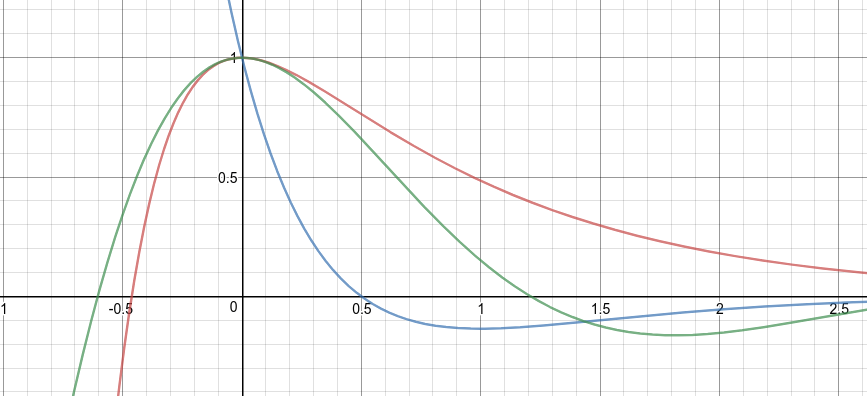
\includegraphics[width=16cm]{assets/hw_06_01.png}
\end{center}

\section*{Section 4.4}

\subsubsection*{Exercise 1}
Decide whether or not the method of undetermined coefficients can be applied to
find a particular solution of the given equation.
\[ y''+2y'-y = t^{-1}\e^t \]
\( \frac{\e^t}{t} \) cannot be formed as \( Ct^m\e^{rt} \), so the method of
undetermined coefficients cannot be applied.

\subsubsection*{Exercise 4}
Decide whether or not the method of undetermined coefficients can be applied to
find a particular solution of the given equation.
\[ x''+5x'-3x = 3^t \]
\( 3^t \) can be rewritten as \( \e^{\ln(3)t} \), so the method of undetermined
coefficients can be applied.

\subsubsection*{Exercise 5}
Decide whether or not the method of undetermined coefficients can be applied to
find a particular solution of the given equation.
\[ y''(\theta)+3y'(\theta)-y(\theta) = \sec(\theta) \]
\( \sec\theta = \frac{1}{\cos\theta} \) cannot be expressed as a product of
polynomials, expoentials, and \( \sin,\cos \), so the method of undetermined
coefficients cannot be applied.

\subsubsection*{Exercise 9}
Find a particular solution to the differential equation.
\begin{align*}
  y''+3y &= -9 \\
  y_p &= A \\
  y_p'' &= 0 \\
  0+3A &= -9 \\
  y_p &= A = -3
\end{align*}

\subsubsection*{Exercise 10}
Find a particular solution to the differential equation.
\begin{align*}
  y''+2y'-y &= 10 \\
  y_p &= A \\
  y_p' &= 0 \\
  y_p'' &= 0 \\
  0-0-A &= 10 \\
  y_p &= A = -10
\end{align*}

\subsubsection*{Exercise 12}
Find a particular solution to the differential equation.
\begin{align*}
  2x'+x &= 3t^2 \\
  x_p &= At^2+Bt+C \\
  x_p' &= 2At+B \\
  2(2At+B)+At^2+Bt+C &= 3t^2 \\
  4At+2B+At^2+Bt+C &= 3t^2 \\
  At^2+(4A+B)t+(2B+C) &= 3t^2 \\
  A &= 3 \quad 4A+B = 0 \quad 2B+C = 0 \\
  A &= 3 \quad B = -12 \quad c = 24 \\
  x_p &= 3t^2-12t+24
\end{align*}

\subsubsection*{Exercise 14}
Find a particular solution to the differential equation.
\begin{align*}
  2z''+z &= 9\e^{2t} \\
  z_p &= A\e^{2t} \\
  z_p' &= 2A\e^{2t} \\
  z_p'' &= 4A\e^{2t} \\
  2(4A\e^{2t})+A\e^{2t} &= 9\e^{2t} \\
  8A+A &= 9 \\
  A &= 1 \\
  z_p &= \e^{2t}
\end{align*}

\subsubsection*{Exercise 18}
Find a particular solution to the differential equation.
\begin{align*}
  y''-2y'+y &= 8\e^t \\
  y_p &= y_p' = y_p'' = A\e^t \\
  A\e^t-2(A\e^t)+A\e^t &= 8\e^t \\
  0 &= 8\e^t
\end{align*}
This does not work since the auxiliary equation \( r^2-2r+1 \) has the double
root \( r = 1 \).
\begin{align*}
  y_p &= At^2\e^t \\
  y_p' &= At^2\e^t+2At\e^t = \e^t(At^2+2At)\\
  y_p'' &= At^2\e^t+2At\e^t+2At\e^t+2A\e^t \\
  &= \e^t(At^2+4At+2A) \\
  \e^t(At^2+4At+2A)-2(At^2\e^t+2At\e^t)+At^2\e^t &= 8\e^t \\
  At^2+4At+2A-2At^2-4At+At^2 &= 8\\
  2A &= 8 \\
  A &= 4 \\
  y_p &= 4t^2\e^t
\end{align*}

\subsubsection*{Exercise 23}
Find a particular solution to the differential equation.
\begin{align*}
  y''(\theta)-7y'(\theta) &= \theta^2 \\
  r^2-7r &= 0 \\
  r &= 0 \quad r = 7 \\
  y''(\theta)-7y'(\theta) &= 1\theta^2\e^{0t} \\
  y_p &= \theta(A\theta^2+B\theta+C) \\
  y_p' &= 3A\theta^2+2B\theta+C \\
  y_p'' &= 6A\theta+2B \\
  6A\theta+2B-7(3A\theta^2+2B\theta+C) &= \theta^2 \\
  -21A\theta^2+(6A-14B)\theta+(6A+2B-7C) &= \theta^2 \\
  -21A &= 1 \quad 6A-14B = 0 \quad 2B-7C = 0 \\
  A &= -\frac{1}{21} \quad B = -\frac{1}{49} \quad C = -\frac{2}{343} \\
  y_p &= -\frac{\theta^3}{21}-\frac{\theta^2}{49}-\frac{2\theta}{343}
\end{align*}

\subsubsection*{Exercise 28}
Determine the form of a particular solution for the differential equation.
\begin{align*}
  y''-6y'+9y &= 5t^6\e^{3t} \\
  C = 5 \quad m &= 6 \quad r = 3 \\
  r^2-6r+9 &= 0 \\
  (r-3)^3 &= 0 \\
  r &= 3 \\
  y_p(t) &= t^2(At^6+Bt^5+Ct^4+Dt^3+Et^2+Ft+G)\e^{rt}
\end{align*}

\begin{center}
  If you have any questions, comments, or concerns, please contact me at
  alvin@omgimanerd.tech
\end{center}

\end{document}
